%%%%%%%%%%%%%%%%%%%%%%%%%%%%%%%%%%%%%%%%%
% Rapport sur package R6
% Version 1 (14/11/2024)
%
% Auteurs :
% Linh Nhi Le Dinh
% Antoine Oruezabala
% Béranger Thomas
%
%%%%%%%%%%%%%%%%%%%%%%%%%%%%%%%%%%%%%%%%%

%----------------------------------------------------------------------------------------
%	Packages
%----------------------------------------------------------------------------------------

\documentclass[10pt,french]{report}

\usepackage[frenchb]{babel}
% Pour les guillemets en style français
\usepackage[french=guillemets]{csquotes}

% Saisir des caractères spéciaux et accentués
\usepackage[utf8]{inputenc}
% Imprimer des caractères spéciaux et accentués
\usepackage[T1]{fontenc}

% Améliorer les espacements
\usepackage{microtype}

\usepackage[a4paper, portrait]{geometry}

% Pour faire des tableaux plus efficacement
\usepackage{tabularray}

% Pour les symboles des équations mathématiques
\usepackage{mathtools}
\usepackage{amssymb}

% Pour charger et afficher des images
\usepackage{graphicx}
\graphicspath{{images/}}


% Pour représenter l'arborescence du programme
\usepackage{dirtree}


% Gérer les espaces entre paragraphes plus facilement
\usepackage{parskip}
\setlength\parindent{0pt}


% Polices de caractères
\usepackage{lmodern}
%\usepackage{stix2} % font stix 2
\usepackage{palatino} % font Palatino


% Pour créer des conditions dans les commandes customisées
\usepackage{ifthen}


% Commande customisée pour dessiner un cube noir, pour faire séparateur
\newcommand{\cube}{\raisebox{0.13ex}{\scalebox{0.75}{ $\blacksquare$ }}}


% Commande customisée pour les entrées du lexique
\newcommand{\entreelex}[3][]{%
	{\large \textbf{\textsc{#2}}} % Entrée (obligatoire)
	\if\relax\detokenize{#1}\relax % Si #1 est vide
	\else % Si #1 n'est pas vide
	\raisebox{0.15ex}{\scalebox{0.7}{$\Diamond$}} % Diamant
	[#1] % Acronyme (facultatif)
	\fi
	\raisebox{0.13ex}{\scalebox{0.75}{$\blacksquare$}} #3 % Définition (obligatoire)
}


% Bibliographie : faire F5, puis F8, puis F5 à nouveau (c'est Latex, c'est tout simple)
\usepackage[style=numeric]{biblatex}
\addbibresource{Rapport.bib}


% Pour faire des hyperliens
\usepackage[colorlinks=true, linkcolor=NavyBlue]{hyperref}
% et leur donner une couleur plus sympa que le bleu habituel
\usepackage[dvipsnames]{xcolor}
\hypersetup{colorlinks=true, citecolor=NavyBlue}

%----------------------------------------------------------------------------------------

\begin{document}

	\begin{titlepage}
		\centering
		\includegraphics[width=0.6\textwidth]{icom.png}\par\vspace{0.5cm}
		{\Large\bfseries Université Lumière Lyon 2}\par
        \par\vspace{3.5cm}



		{\Huge\bfseries Librairie MIMOSA}\par\vspace{0.75cm}
		{\huge\bfseries Mixed Input Multinomial Optimization for Statistical Analysis}\par\vspace{0.75cm}

		{\Large\itshape Régression logistique multinomiale sur données mixtes,\\par descente de gradient}\par\vspace{3.5cm}

		{\Large\itshape Par}\par
		{\Large Linh Nhi Le Dinh}\par
		{\Large Antoine Oruezabala}\par
		{\Large Béranger Thomas}\par\vspace{1cm}

		{\large\itshape Rapport présenté dans le cadre du}\par
		{\large Master 2 SISE - Promotion 2024/2025}\par\vspace{1cm}

		\vfill

	\end{titlepage}

	\tableofcontents

	\setlength{\parskip}{12pt}

	\begin{abstract}
		Ce rapport détaille l'implémentation de la régression logistique multinomiale pour des données mixtes, en langage R, et en utilisant la descente de gradient. Nous couvrons tout d'abord quelques fondements théoriques, puis l'approche pratique et enfin discutons des résultats obtenus. En fin d'ouvrage, un lexique donne une définition des termes et expressions souvent usité en régression logistique.

		Ce rapport a été rédigé en novembre 2024 dans le cadre d'un projet du master 2 SISE.
	\end{abstract}

	\chapter{Théorie}

	\section{La régression logistique multinomiale}
	\subsection{Principes Généraux}
	% Description du modèle multinomial et de ses applications.
	La régression logistique vise à prédire la probabilité qu'un événement binaire se produise (oui/non, 1/0) en fonction de variables explicatives. Elle utilise une fonction logistique (ou sigmoïde) pour transformer la combinaison linéaire des variables explicatives en une probabilité comprise entre 0 et 1.

	La régression logistique \textbf{multinomiale} est une généralisation de la régression logistique binaire. Elle permet d'estimer la probabilité d'appartenance à chacune des catégories en fonction de variables explicatives quantitatives et/ou qualitatives. Contrairement à la régression logistique binaire qui modélise une seule probabilité $p$, la régression logistique multinomiale estime simultanément les probabilités d'appartenance à toutes les catégories ($p_1, p_2, ..., p_K$), avec la contrainte que leur somme soit égale à 1.

	Le modèle utilise une transformation logistique qui garantit que les probabilités estimées restent comprises entre 0 et 1. Une catégorie est choisie comme référence, et le modèle estime les logarithmes des rapports de probabilités (log-odds) entre chaque catégorie et cette référence.

	Nous nous placerons dans le cas où cette régression est nominale, c'est-à-dire que l'on ne suppose aucun ordre particulier entre les modalités de la variable à prédire.

    \subsection{Modélisation mathématique}

    Pour construire un modèle de régression logistique, l'équation de régression linéaire est utilisée comme point de départ\cite{datatab, ricco} :

     \begin{equation}
         \hat{y} = a + b_1x_1 + \ldots + b_kx_k
     \end{equation}

     Avec :
     \begin{itemize}
         \item $\hat{y}$ la variable cible
         \item $a$ l'intercept,
         \item $x_k$ la variable prédictive $k$,
         \item $b_k$ le coefficient rattaché à cette variable,
         \item $K$ le nombre de variables prédictives.
     \end{itemize}

    Toutefois, une telle équation produirait des coefficients $\in \mathbb{R}$, et l'objectif de la régression logistique est d'estimer la probabilité d'occurrence et non la valeur de la variable elle-même. Cette équation doit donc être transformée.

    C'est le rôle de la fonction LOGIT.

	\subsection{Fonction de Coût}
	% Explication de la fonction d'erreur cross-entropy catégorielle.
	La fonction de coût utilisée pour la régression logistique multinomiale est la cross-entropie catégorielle. Elle évalue la divergence entre les probabilités prédites par le modèle et les probabilités réelles des classes. Elle est définie comme suit :

	\[
	J(\beta) = -\frac{1}{N} \sum_{i=1}^{N} \sum_{k=1}^{K} y_{i,k} \log\left( P(Y = k \mid X_i) \right)
	\]

	où :

	- \( N \) est le nombre total d'observations.
	- \( K \) est le nombre de classes.
	- \( y_{i,k} \) est une variable indicatrice qui vaut 1 si l'observation \( i \) appartient à la classe \( k \), et 0 sinon.
	- \( P(Y = k \mid X_i) \) est la probabilité prédite que l'observation \( i \) appartienne à la classe \( k \).

	Minimiser cette fonction de coût permet d'ajuster les paramètres \( \beta \) du modèle pour améliorer la précision des prédictions. La descente de gradient est une méthode d'optimisation utilisée pour trouver les valeurs optimales de \( \beta \) qui minimisent \( J(\beta) \).

	\subsection{Hypothèses du Modèle}
	% Discussion sur l'utilisation de la fonction SoftMax.
	Dans le cadre de la régression logistique multinomiale, plusieurs hypothèses fondamentales sont posées pour assurer la validité et la robustesse du modèle :

	\begin{itemize}
		\item \textbf{Indépendance des observations} : Chaque observation est supposée indépendante des autres. Cette hypothèse garantit que l'information apportée par chaque donnée est unique et non redondante.

		\item \textbf{Relation linéaire entre les variables explicatives et le logit} : Le modèle suppose une relation linéaire entre les variables explicatives \( X \) et le logarithme des probabilités conditionnelles (logits). Cela signifie que l'effet de chaque variable explicative est additif sur le logit.

		\item \textbf{Absence de multicolinéarité parfaite} : Les variables explicatives ne doivent pas être des combinaisons linéaires exactes les unes des autres. La présence de multicolinéarité peut entraîner des estimations instables des coefficients du modèle.

		\item \textbf{Catégories mutuellement exclusives et exhaustives} : Les classes de la variable dépendante doivent être clairement définies sans chevauchement, et couvrir toutes les possibilités.

	\end{itemize}

	La fonction \textit{SoftMax} est essentielle dans ce modèle car elle transforme les scores linéaires en probabilités. Elle garantit que les sorties du modèle sont comprises entre 0 et 1 et que la somme des probabilités pour toutes les classes est égale à 1 pour chaque observation. La fonction \textit{SoftMax} est définie par :

	\[
	P(Y = k \mid X) = \frac{\exp(X\beta_k)}{\sum_{j=1}^K \exp(X\beta_j)}
	\]

	où \( K \) est le nombre total de classes. Cette transformation est basée sur l'hypothèse que les logits peuvent être exponentiés et normalisés pour obtenir des probabilités, ce qui est cohérent avec le principe de maximum d'entropie.

	L'utilisation de la fonction \textit{SoftMax} implique également que les classes sont mutuellement exclusives, ce qui signifie qu'une observation ne peut appartenir qu'à une seule classe. Cela correspond à la nature des problèmes de classification multinomiale où le but est de prédire une seule catégorie parmi plusieurs possibles.

	\section{L'algorithme de descente de gradient}

	La descente de gradient est un algorithme d’optimisation itératif, qui permet de trouver le minimum d'une fonction.

	L'idée est la suivante :
	\begin{itemize}
		\item on part d'un point choisi aléatoirement,
		\item depuis ce point nous cherchons le gradient (la pente),
		\item et nous descendons d'un pas dans la direction opposé au gradient,
		\item nous recommençons le processus à partir du nouveau point atteint.
	\end{itemize}

	Les critères pour s'arrêter peuvent être :
	\begin{itemize}
		\item le nombre d'itérations; on définit un maximum au début de l'algorithme, que l'on ne dépasse pas,
		\item la différence de "niveau" entre deux points; si elle passe en dessous d'un seuil très faible, l'approximation est jugée suffisamment bonne,
		\item une combinaison de ces deux critères, qui a l'avantage de s'arrêter le plus tôt possible.
	\end{itemize}

	Vocabulaire :
	\begin{itemize}
		\item la taille du pas est dénommé taux d'apprentissage (en anglais learning rate),
		\item la différence minimale souhaitée entre deux points consécutifs est la tolérance,
		\item
		\item
	\end{itemize}
	Mathématiquement, la pente est définie par le gradient. La taille du pas est dénommé taux d'apprentissage.

	La pente, forte au départ forte, doit aller en décroissant au fur et à mesure que l'on se rapproche du point le plus bas (ou d'un minimum local). On peut, pour limiter le temps de calcul, définir une différence minimale entre deux points consécutifs en-dessous de laquelle il n'est pas utile d'entamer une nouvelle itération. Cette différence minimale s'appelle la tolérance.

	Il existe trois types d'algorithmes d'apprentissage par descente de gradient : la descente de gradient simple (sur tous les points), la descente de gradient stochastique et la descente de gradient par mini-lots.

	\subsection{Modélisation}

	\subsection{Test}

	\chapter{Implémentation Pratique en R}

	\section{Structure du programme}

	L'architecture du programme est la suivante :

	\dirtree{%
		.1 {projet\textunderscore racine/}.
		.2 {datasets/}.
		.2 {docs/}.
		.3 {Rapport.pdf}.
		.3 {Rapport.tex}.
		.2 {utils/}.
		.3 {LogisticRegression.r}.
		.3 {preprocessing.r}.
		.3 {utils.r}.
		.2 {main.r}.
	}

	Les fichiers sont décrits ci-après, avec du pseudo-code pour certaines fonctions.

	\subsection{main.r}

	Le fichier \texttt{main.r} contient le programme principal, qui instancie l'objet \texttt{LogisticRegression}, qui contient les fonctions suivantes :

	\begin{itemize}
		\item \texttt{fit} : pour modéliser
		\item \texttt{transform} : pour
		\item \texttt{probas}
	\end{itemize}

	\subsection{utils.r}

	Le fichier \texttt{utils.r} contient une fonction \textit{check\textunderscore type}, qui vérifie si l'objet passé en premier argument est du même type que le type passé en second argument.

	Si ce n'est pas le cas, le programme s'arrête.

	\subsection{preprocessing.r}

	Le fichier \texttt{preprocessing.r} contient plusieurs fonctions de prétraitement :

	\begin{itemize}
		\item imputer\textunderscore numeriques : réalise une imputation par la moyenne des valeurs manquantes dans le jeu de données passé en argument.
		\item imputer\textunderscore categorielles : réalise une imputation par le mode des valeurs manquantes dans le jeu de données passé en argument.
		\item split\textunderscore train\textunderscore test : réalise une séparation du jeu de données passé en argument
	\end{itemize}

	\subsection{LogisticRegression.r}

	Le fichier \texttt{LogisticRegression.r} contient toutes les fonctions nécessaires à la réalisation de la régression logistique :

	\subsubsection{Fonction \enquote*{sigmoid}}
	Applique la \hyperref[fonction sigmoïde]{fonction sigmoïde} à la valeur passée en argument et renvoie le résultat.

	\subsubsection{Fonction \enquote*{softmax}}
	Applique la \hyperref[fonction softmax]{fonction softmax} à la valeur passée en argument et renvoie le résultat.

	\subsubsection{Fonction \enquote*{cout}}
	Fonction de coût pour la régression logistique, avec cross-entropy :

	\begin{verbatim}
		cout <- function(X, y, beta) {
			   n <- nrow(X)
			   scores <- X %*% beta
			   probs <- exp(scores) / rowSums(exp(scores))
			   cost <- -mean(sum(y * log(probs)))
			   return(cost)
		    }
	\end{verbatim}

	\subsubsection{Fonction \enquote*{hypothese}}

	\subsubsection{Fonction \enquote*{descente\textunderscore gradient}}

	Applique une descente de gradient pour la régression logistique :
	\begin{verbatim}
		descente_gradient <- function(X, y, beta) {
			n <- nrow(X)
			scores <- X %*% beta
			probs <- exp(scores) / rowSums(exp(scores))
			gradient <- -t(X) %*% (y - probs) / n
			return(gradient)
		}
	\end{verbatim}

	\subsection{Répertoire docs}

	Il contient :
	\begin{itemize}
		\item ce rapport au format pdf : \texttt{Rapport.pdf},
		\item et au format Latex : \texttt{Rapport.tex}
	\end{itemize}

	\section{Vérification des données}
	% Inclus dans le initialize, c'est-à-dire appelé lors de l'instanciation de l'objet LogisticRegression
	Afin de s'assurer de l'intégrité des données, nous procédons à plusieurs vérifications lors de l'instanciation de l'objet \textit{LogisticRegression}.

	\subsection{Format des objets passés en argument}

	Les deux vérifications suivantes sont réalisées à l'aide de la fonction \textit{check\textunderscore type} du fichier \textit{utils.r} :

	\begin{enumerate}
		\item les données explicatives $X$ doivent être dans un data.frame
		\item la cible $y$ doit être un vecteur ou un character
	\end{enumerate}

	\subsection{Format des données}

	\begin{enumerate}
		\item Les données de la cible $y$ doivent être de type catégorielle (character ou factor).
	\end{enumerate}

	\subsection{Cohérence des données}

	\begin{enumerate}
		\item La cible $y$ doit être présente dans les données $X$,
		\item il faut au moins deux modalités pour la variable cible $y$.
	\end{enumerate}

	\section{Pré-traitement des données}
	% Étapes de traitement des données avant modélisation.

	\subsection{Variable cible $y$}

	Si le format des données de la variable cible ne correspondaient pas aux pré-requis (variable catégorielle et avec au moins deux modalités), le programme l'aura signalé lors de l'instanciation de l'objet \textit{LogisticRegression}.

	Il n'y a pas d'autre contrainte à respecter pour la variable cible $y$, mais une opération de suppression des lignes sans la variable cible est mené ici. Le but étant bien évidemment de ne pas charger à modéliser sur des données manquantes pour a cible, ce qui n'aurait pas de sens puisque nous sommes en apprentissage supervisé.

	\subsection{Variables explicatives $X$}

	Les variables explicatives peuvent être mixtes, numériques et/ou catégorielles. Dans les deux cas, des pré-traitements sont nécessaires.

	\subsubsection{Variables numériques}

	Afin de pouvoir comparer des données aux unités quelques fois différentes, on centre et réduit les données numériques. Les coefficients seront alors normalisés ce qui permettra leur comparaison directe.

	\subsubsection{Variables catégorielles}

	Chaque variable catégorielle subit deux étapes pour les préparer à la descente de gradient :

	\begin{enumerate}
		\item un \textit{codage disjonctif} (one-hot encoding) pour produire des valeurs numériques,
		\item la suppression d'une des modalités.
	\end{enumerate}

	Cette dernière étape permet d'éviter la colinéarité, c'est-à-dire la redondance d'information entre variables (une variable désignant ici une des colonnes produites par le one-hot encoding; c'est-à-dire une des modalités de la variable encodée).
	%

	\chapter{Éléments introductifs}

	\section{La régression logistique}

	Quelle soit binaire (la variable cible possède deux modalités) ou multinomiale (la variable cible possède plus de deux modalités), le principe de la régression logistique est de maximiser la vraisemblance, ou pour le dire autrement, de minimiser la déviance.

	Quel outil pour mesurer ce paramètre ? La log-vraisemblance.

    \subsection{Notations}

    Soit une population $\Omega$ de $n$ individus, définie par $J$ variables explicatives notées $\left\{X_{1}, \ldots,X_{J}\right\}$, et une variable cible $Y$ possédant $K$ valeurs :

    \begin{tblr}{
            colspec = {X[4,c]X[4,c]X[4,c]X[4,c]X[4,c]},
            rowspec = {Q[m]Q[m]Q[m]Q[m]Q[m]},
            rowsep = 5pt,
            hlines,
            vlines,
        }
        $\Omega$ & Cible & $X_{1}$ & $\ldots$ & $X_{J}$ \\
        1 & $Y_{1}$ &  &  &  \\
        $\ldots$ & $\ldots$ &  &  &  \\
        $\omega$ & $Y_{\omega}$ & $X_{1}\left(\omega\right)$ & $\ldots$ & $X_{J}\left(\omega\right)$ \\
        $\ldots$ & $\ldots$ &  &  &  \\
        $n$ & $Y_{K}$ &  &  &  \\
    \end{tblr}

    Dans le cas binaire, la probabilité d'un individu $\omega$ d'être positif à priori se note $p$ par commodité, pour simplifier $p\left(\omega\right)$, lui-même une notation simplifiée de $P\left[Y\left(\omega\right)=+\right]$.

    Toujours dans le cas binaire, la probabilité d'un individu $\omega$ d'être positif à posteriori, c'est-à-dire la probabilité que l'on modélisera en apprentissage supervisée, se note $\pi$ par commodité, pour simplifier $\pi\left(\omega\right)$, lui-même une notation simplifiée de $P\left[Y\left(\omega\right)=+/X\left(\omega\right)\right]$.

    La fonction LOGIT pour cet individu $\omega$ est :

    \begin{equation}
        \text{LOGIT}(\omega) = \ln\left[\frac{\pi(\omega)}{1-\pi(\omega)}\right] = a_0 + a_1X_1\left(\omega\right) + \cdots + a_JX_J\left(\omega\right)
    \end{equation}

    Soit en écriture matricielle :

    \begin{equation}
        \ln\left[\frac{\pi(\omega)}{1-\pi(\omega)}\right] = X\left(\omega\right) \times a
    \end{equation}

    Avec $a_0, \ldots, a_J$ les paramètres que l'on souhaite estimer.

	\subsection{Algorithmes}

    Un algorithme utilisé pour optimiser la log-vraisemblance est celui de Newton-Raphson. Il s'agit d'une approche itérative, qui utilise la dérivée de la fonction considérée pour approcher une solution.

    Il a toutefois pour défaut d'utiliser la matrice hessienne, qui peut être coûteuse en mémoire et temps de calcul.

    Nous expliquerons et utiliserons un autre algorithme ici, la descente de gradient.

    Il s'agit aussi d'un algorithme itératif, dont l'objectif est de trouver le minimum d'une fonction $f\left(x\right)$ en partant d'un point arbitraire $x_0$. On se \enquote{déplace} pour cela dans la direction opposée au gradient, c'est-à-dire que l'on \enquote{descend} le long de la pente.

    Mathématiquement, on part d'une valeur arbitraire $x_0$, puis pour trouver $x_1$ on utilise la formule suivante :

    \begin{equation}
        x_{n+1} = x_n - \alpha \nabla f\left(x_n\right)
    \end{equation}

    Avec :
    \begin{itemize}
        \item $x_n$ la position actuelle,
        \item $\alpha$ le taux d'apprentissage,
        \item $\nabla f\left(x_n\right)$ le gradient de la fonction au point $x_n$
    \end{itemize}

    Les étapes sont donc les suivantes :
    \begin{itemize}
        \item choisir un point $x_0$ arbitraire pour commencer les calculs,
        \item calculer le gradient à ce point,
        \item mettre à jour la position en se déplaçant dans la direction opposée,
        \item vérifier que l'on a atteint un critère d'arrêt :
        \begin{itemize}
            \item nombre d'itérations maximum atteint,
            \item et/ou précision souhaitée (différence entre deux itérations) atteinte,
        \end{itemize}
    \end{itemize}

	\subsection{Champs d'application}

    La régression logistique n'émet pas d'hypothèse directement sur les distributions des probabilités $P\left(X/Y=+\right)$ et $P\left(X/Y=-\right)$, mais uniquement sur leur rapport.

    Elle permet donc, en théorie, une application plus large, et est nommé semi-paramétrique, pour la différencier des modèles qui supposent une loi donnée sur la distribution des probabilités.


	\chapter{Lexique}

	\label{Centrage et réduction}
	\entreelex{Centrage et réduction}{L'opération de centrage et réduction transforme les données pour avoir une moyenne de 0 et un écart-type de 1 :

	\begin{equation}
		x_{cr}=\frac{x_{i}-\bar{x}}{\sigma}
	\end{equation}

	 Centrer et réduire les données ne change pas les distributions, seulement l'échelle des données. Le centrage déplace le centre de la distribution au point zéro de l'axe des abscisses, et la réduction modifie l'échelle pour que l'écart-type soit égal à 1.

	 Il rend les variables indépendantes de leur unité de mesure initiale et permet donc de comparer des variables mesurées dans des unités ou sur des échelles différentes.}

	 \label{fonction sigmoïde}
	 \entreelex{Fonction sigmoïde}{La fonction sigmoïde ou logistique s'applique aux nombres réels et est utilisée pour transformer des valeurs réelles en probabilités. Elle produit une courbe en forme de S, avec des valeurs comprises entre 0 et 1.

	 \begin{figure}[h]
	 	\centering
	 	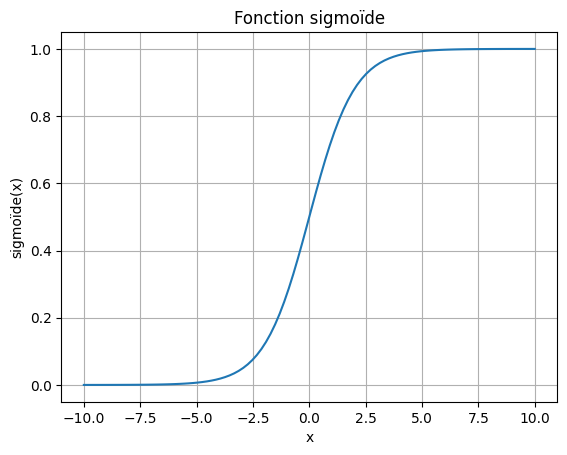
\includegraphics[width=0.6\textwidth]{f_sigmoide.png}
	 	\caption{La fonction sigmoïde}
	 	\label{fig:mesh1}
	 \end{figure}

	 Elle est l'inverse de la fonction LOGIT. Sa formule est :

 	\begin{equation}
 		\sigma(x) = \frac{1}{1 + e^{-x}}
 	\end{equation}

 	Où:
 	\begin{itemize}
 		\item $\sigma(x)$ représente la fonction sigmoïde
 		\item $e$ est la base du logarithme naturel (constante d'Euler)
 		\item $x$ est la variable d'entrée
 	\end{itemize}

 	Les deux fonctions logistique et LOGIT étant inverses l'une de l'autre, cela signifie que :
 	\begin{itemize}
 		\item $\text{logit}(\sigma(x)) = x$
 		\item $\sigma(\text{logit}(p)) = p$
	 \end{itemize}}

	 \label{fonction softmax}
	 \entreelex{Fonction softmax}{La fonction softmax est une fonction d'activation qui transforme un vecteur de nombres réels en une distribution de probabilités.}

	\entreelex{Modalité de référence}{Modalité de référence par rapport à laquelle le LOGIT est exprimé.}

	\label{taux apprentissag}
	\entreelex{Taux d'apprentissage}{Ou learning Rate : il fixe la « grandeur » du pas de chaque itération de la descente de gradient.}

	\entreelex{Descente de gradient}{La descente de gradient est un algorithme d’optimisation couramment utilisé pour entraîner les modèles de machine learning et les réseaux neuronaux. Ce type d’algorithme entraîne les modèles de machine learning par réduction des erreurs entre les résultats prédits et les résultats réels.\cube Le point de départ n'est qu'un point arbitraire qui nous permet d'évaluer les performances. À partir de ce point de départ, nous allons trouver la dérivée (ou la pente) et, à partir de là, nous pourrons utiliser une ligne tangente pour observer l'inclinaison de la pente. La pente renseigne sur les mises à jour des paramètres, c'est-à-dire les poids et les biais. La pente au point de départ est plus forte, mais au fur et à mesure que de nouveaux paramètres sont générés, elle devrait progressivement diminuer jusqu'à atteindre le point le plus bas de la courbe, dénommé point de convergence.\cube Comme pour trouver la ligne de meilleur ajustement dans la régression linéaire, l'objectif de la descente de gradient est de minimiser la fonction de coût, ou l'erreur entre y prédit et y réel. Pour ce faire, deux points de données sont nécessaires : une orientation et un taux d'apprentissage. Ces facteurs déterminent les calculs de dérivée partielle des itérations futures, ce qui lui permet d'atteindre progressivement le minimum local ou global (c'est-à-dire le point de convergence).. La fonction de perte dans la descente de gradient agit spécifiquement comme un baromètre, évaluant sa précision à chaque itération des mises à jour de paramètres. Jusqu'à ce que la fonction soit proche ou égale à zéro, le modèle continue à ajuster ses paramètres pour obtenir l'erreur la plus faible possible.\cube Il existe trois types d'algorithmes d'apprentissage par descente de gradient : la descente de gradient par lots, la descente de gradient stochastique et la descente de gradient par mini-lots.}

	\listoffigures

    \printbibliography

\end{document}
